\section{Roadmap for This Doc}

\begin{enumerate}
\item Improve the roadmap at the end of this document
\item Update the preceeding sections
\item Revise the intro
\item Make it all into a readable paper
\item Submit to PLoP 2015 http://www.hillside.net/plop/2015/
\item Charlie goes on a date with Tonya
\end{enumerate}

\section{Patterns}

\begin{quote}
Although a grounding in learning theory helps inform peer learning
projects, Peeragogy, at its core, comes to life in applied practice.
Even before convening a group for your peer learning project
(discussed in Part IV), you will want to take a look
over the patterns we have collected.  You will likely return here many
times as your project develops.
\end{quote}

\subsection{What is a pattern?}

A pattern is anything that has a repeated effect. In the context of
peeragogy, the practice is to repeat processes and interactions that
advance the learning mission. Frequent occurrences that are not
desirable are called anti-patterns!

\begin{quote}
\textbf{Christopher Alexander}: ``Each pattern describes a problem which
occurs over and over again in our environment, and then describes the
core of the solution to that problem, in a way that you can use this
solution a million times over, without ever doing it the same way
twice.'' {[}1{]}
\end{quote}

Patterns provide a framework that can be applied to similar issues but
may be metaphorically solved in different ways, sometimes in real world
or face to face events and other times in digital space.~ Outside of
Alexander's own work in architecture, one the first groups to adopt a
design pattern way of thinking about things were computer programmers.~
Writing in the foreward to Richard P. Gabriel's \emph{Patterns of
Software}, Alexander emphasizes that the key question to ask about any
design approach is: does it help us build better?

\begin{quote}
\textbf{Christopher Alexander}: ``What is the Chartres of programming?
What task is at a high enough level to inspire people writing programs,
to reach for the stars?'' {[}2{]}
\end{quote}

We think that Peeragogy stands a good chance of being a~``killer app''
for pattern-based design.~ Learning bridges physical and virtual worlds
all the time.~ And, in fact, a \emph{Network of Learning} was the 18th
pattern that Christopher Alexander introduced in his book, \emph{A
Pattern Language}.

\begin{quote}
\textbf{Christopher Alexander}: ``Work in piecemeal ways to decentralize
the process of learning and enrich it through contact with many places
and people all over the city: workshops, teachers at home or walking
through the city, professionals willing to take on the young as helpers,
older children teaching younger children, museums, youth groups
travelling, scholarly seminars, industrial workshops, old people, and so
on.'' {[}1{]}
\end{quote}

Peeragogy can help to extend and enrich this network, and, as we shall
see, patterns can be used by those involved to do ongoing ``emergent''
design, not only by building new structures, but by adapting and
improving our catalog of patterns as we go.~ For consistency, and easy
use, adaptation, and extension we present the patterns using the
following template.~ The format is meant to be neutral and easy to work
with -- it's, intentionally, an outline that you might use to write a
short abstract describing an active project.

\begin{quote}
\textbf{Title}: \emph{Encapsulate the idea - possibly include a
subtitle}

\textbf{Definition}: \emph{Explain the idea and the context in which it
is meaningful. ~(You can link to other patterns, if they are useful for
clarifying the relevant context.)}

\textbf{Problem}: \emph{Explain why there's some issue to address here.}

\textbf{Solution}: \emph{Talk about an idea about how to address the
issue.}

\textbf{Challenges}: \emph{Talk about what can go wrong.}

\textbf{What's Next}: \emph{Talk about specific next steps. ~(Again,
link to other patterns, if they are useful for clarifying the relevant
context.)}

The pattern template also includes the following optional elements:

{[}\textbf{Objectives}: \emph{Explain the purpose(s) of the proposed
solution's functioning, if they aren't fully specified by the
description of the solution itself.}{]}

{[}\textbf{Examples}: \emph{Present example(s) that have been
encountered, if this aids comprehension.}{]}

{[}\textbf{References}: \emph{Citations, if relevant.}{]}
\end{quote}

Notice the emphasis the active aspect of things -- the ``What's Next''
section concretely links the patterns we discuss here to the Peeragogy
project.~ If you adapt them for use in your own project, you're likely
to have a different set of next steps. Although we think that these
patterns can be generally useful, they aren't useful in the abstract,
but rather, as a way for discussing what we actually do.

\subsection{Patterns of peeragogy}

Here is our index of the main patterns we've found so far (described in
more detail after the jump):

\begin{itemize}
\itemsep1pt\parskip0pt\parsep0pt
\item
  \href{http://peeragogy.org/patterns/wrapper/}{Wrapper} - Front end
  appearance to participants. Consolidate and summarize.
\item
  \href{http://peeragogy.org/patterns/discerning-a-pattern/}{Discerning
  a pattern} - Found a pattern? Give it a title and record an example.
  (Woah, meta!)
\item
  \href{http://peeragogy.org/patterns/polling-for-ideas/}{Polling for
  ideas} - Invite brainstorming, collecting ideas, questions, and
  solutions.
\item
  \href{http://peeragogy.org/patterns/creating-a-guide/}{Creating a
  guide} - Overviews expose the lay of the land. Collecting content and
  stories.
\item
  \href{http://peeragogy.org/patterns/newcomer/}{Newcomer} - Create a
  guide for ``beginner's mind'' and help avoid need to introduce new
  members each ``meeting.''
\item
  \href{http://peeragogy.org/patterns/roadmap/}{Roadmap} - Plans for
  future work, direction towards a goal, dynamic
\item
  \href{http://peeragogy.org/patterns/roles/}{Roles} - Specialize and
  mix it up. Play to participants strengths and skills.
\item
  \href{http://peeragogy.org/focusing-on-a-specific-project/}{Project
  focus} - Lightbulb moment: Most specific projects involve learning!
\item
  \href{http://peeragogy.org/patterns/carrying-capacity/}{Carrying
  capacity} - Know your limits, find ways to get other people involved.
\item
  \href{http://peeragogy.org/patterns/heartbeat/}{Heartbeat} - The
  ``heartbeat'' of the group keeps energy flowing.
\item
  \href{http://peeragogy.org/patterns/moderation/}{Moderation} - When
  leaders step back, dynamics can improve; moderator serves as champion
  and editor.
\item
  \href{http://peeragogy.org/patterns/praxis-vs-poeisis/}{Use or make?}
  - Repurposing, tinkering, or creating from scratch?
\end{itemize}

We'll introduce one more pattern in a short
\href{http://peeragogy.org/case-study-learning-to-use-technology-with-peers-the-case-of-swats/}{case
  study} that appears in Chapter \ref{swats}.

\subsection{Anti-patterns for Peeragogy}

And some ``anti-patterns'' (things to avoid if possible).~ Note that we
use the same template to talk about both patterns and anti-patterns, but
here, although the proposed solution may look like a good idea
initially, but it doesn't work so well over the long term. Pay
particular attention to the challenges that arise in practice!

\begin{itemize}
\itemsep1pt\parskip0pt\parsep0pt
\item
  \href{http://peeragogy.org/antipatterns/isolation/}{Isolation} -~ A
  tale of silos, holes, and not-invented-here.
\item
  \href{http://peeragogy.org/antipatterns/magical-thinking/}{Magical
  thinking} - ~``One meeting will (not) change everything!''
\item
  \href{http://peeragogy.org/antipatterns/co-learning-messy-with-lurkers/}{Messy
  with Lurkers} - What happens when joining is low-cost and completion
  is low-benefit.
\item
  \href{http://peeragogy.org/antipatterns/misunderstanding-power/}{Misunderstanding
  Power} - The workload is almost never evenly distributed.
\item
  \href{http://peeragogy.org/antipatterns/navel-gazing/}{Navel Gazing} -
  ``I have this really great idea\ldots{}''
\item
  \href{http://peeragogy.org/antipatterns/stasis/}{Stasis} - What is the
  driver behind open source, commons-oriented collaborative projects?~
  (Because, let's face it, it doesn't always work.)
\item
  \href{http://peeragogy.org/antipatterns/stuck-at-the-level-of-weak-ties/}{Stuck
  at the level of weak ties} - Can we deepen the connection?
\end{itemize}

%% \subsection{What is a use case?}

%% A use case describes someone (or something) who uses a given system or
%% tool to achieve a goal. A use case can include a title, a summary of the
%% problem, an actor, and a success scenario. Additional features can be
%% added, such as alternate interactions or choices that lead to a
%% variation on the result.

%% The use case considers a given persona (a characteristic role) in a
%% given situation and shows how they works on a project/problem and how
%% their process of work is resolved into a solution or solutions. Some
%% activities do not have a single solution -- these are often referred to
%% as ``Wicked Problems.''~ With detailed bookkeeping effort, recorded
%% processes can be standardized into use cases that can then be employed
%% directly or modified to fit the context of the activity at hand.~ In
%% short, they are a lot like design patterns, which they may contain in
%% hidden or explicit form. Use cases are presented in vignettes that
%% appear throughout the book (like the one at the end of this section).

\subsection{A peeragogy pattern language}

By looking at how patterns combine in real and hypothetical use cases,
you can start to identify a \emph{pattern language} that can be used in
your projects. We can get a simplified view of these connections with
the following diagram.~ It's important to clarify that everyone doesn't
do it the same way.~ Here, the \emph{Roadmap} is given a central
position, but some peer learning projects will forego making a specific,
detailed plan; their plan is just to see what develops. You can see here
how peeragogy patterns often break down further into individual
micro-steps: we'll say more about that shortly.

% {\centering 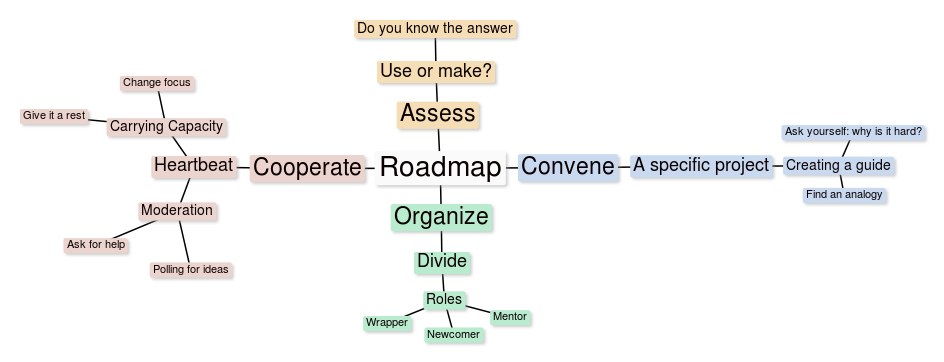
\includegraphics[width=\textwidth]{../pictures/pattern-language.jpg}\par}

The subsequent main sections of this book --
\href{http://peeragogy.org/convene/}{\emph{Convene}},
\href{http://peeragogy.org/organize/}{\emph{Organize}},
\href{http://peeragogy.org/facilitate/}{\emph{Cooperate}} and
\href{http://peeragogy.org/assessment/}{\emph{Assess}} -- represent big
clusters of patterns that are likely to come up time and again in
various projects.~ We can think of these as East, South, West, and North
in the diagram above. You are of course encouraged to invent your own
patterns and to connect them in new ways. Each project has a unique
design, and it's own unique way in which things play out in practice.~
What we've put together here is a starter kit.

\begin{quote}
\textbf{Christopher Alexander}: ``These ideas---patterns---are hardly more
than glimpses of a much deeper level of structure, and is ultimately
within this deeper level of structure, that the origin of life occurs.''
{[}2{]}
\end{quote}

\noindent The peeragogy patterns suggest a \emph{social} way to implement useful problem-solving heuristics [3]:

\begin{itemize}
\itemsep1pt\parskip0pt\parsep0pt
\item
  We simplify things for \textbf{Newcomers}. We don't expect a newcomer to
  enter at full speed.
\item
  We use a~\textbf{Roadmap} to guide us from one phase to another, while
  the project's central~\textbf{Heartbeat}~helps us attend to the
  central focus.
\item
  We announce significant changes through a \textbf{Wrapper} who
  describes any new directions taken by the project.
\item
  We divide work up not only horizontally among different
  \textbf{Roles}, but also temporally by using the \textbf{Roadmap}.
\item
  Whenever we're \textbf{Creating a Guide}
  we're really thinking in terms of analogies.
\item
  When we ask for help, we often avail ourselves of some sort of
  \textbf{Moderation}.
\item One simple way to ask for help is \textbf{Polling for Ideas}.
\item
  If you know the answer (or if you know someone who knows), then you may be able to reuse it.  We often reuse instead of making-anew: ask ``\textbf{Use or Make}?''
\item
  It is important to give it a rest so as not to exhaust one's own
  \textbf{Carrying Capacity} -- or get too far out of sync with the
  group.
\item One of the things that experts are good at is \textbf{Discerning
  a Pattern}. This allows them to simplify their processing.  We like to describe and share the patterns we find.
\item If we know why something is hard, then we may be able to use
  that information to \textbf{Create a Guide} that will help get
  around, or at least better cope with, the difficulty.
\end{itemize}

\subsubsection{References}

\begin{enumerate}
\itemsep1pt\parskip0pt\parsep0pt
\item
  Alexander, C., Ishikawa, S., and Silverstein, M. (1977). \emph{A
  Pattern Language: Towns, Buildings, and, Construction}, New York:
  Oxford University Press.
\item
  Gabriel, Richard P. (1996).
  \emph{\href{http://dreamsongs.net/Files/PatternsOfSoftware.pdf}{Patterns
  of Software}}, New York: Oxford University Press. (Includes a foreward
  by Christopher Alexander.)

\item Minsky, Marvin. (2008--2009). \emph{Essays on Education (for {O}{L}{P}{C})}, Massachusetts Institute of Technology Media Lab whitepaper, \href{http://web.media.mit.edu/~minsky/OLPC-1.html}{Available online.}
\end{enumerate}
